\chapter{Diseño}

En este capítulo se abordarán las cuestiones de diseño la interfaz de usuario, explicando de manera detallada cada elemento que la compone, junto a algunos bocetos. Además, se incluirá un diagrama de navegación para saber a qué pantallas lleva cada opción, una explicación de todas las entidades y atributos, junto a un diagrama de clases del sistema.

\bigskip

Cada cuestión anteriormente mencionada se dividirá en secciones a continuación:

\section{Modificación del estado de los pilotos}
El estado de los pilotos viene determinado por los siguientes parámetros:

\begin{itemize}
    \item \textbf{Experiencia: }El valor se encuentra en el intervalo [0,1] y solo podrá ser modificado mediante el configurador. Determinará la velocidad con la que se reduce el aguante, lo que significa que para valores de experiencia más altos, el aguante disminuirá más lentamente. También influirá en la velocidad de acumulación y pérdida (Sección \ref{sec:componente-estado}) de agresividad, de modo que para valores más altos de experiencia, la agresividad aumentará más lentamente y disminuirá más rápidamente.
    
    \item \textbf{Aguante físico y mental: }El valor se encuentra en el intervalo [0,1], donde 0 representa el mínimo aguante y 1 el mayor. Todos los pilotos comenzarán con el valor máximo, que es 1. Un valor elevado de aguante permite al piloto tener buen ritmo en las curvas (Sección \ref{sec:componente-estado}), mientras que un valor bajo de aguante provoca una disminución en el ritmo; es decir, puede perder hasta un máximo de 20 km/h en las curvas. Cabe destacar que este valor disminuye periódicamente para todos los pilotos, y la velocidad de pérdida puede variar en función de la experiencia.
    
    \item \textbf{Agresividad: }El valor se encuentra en el intervalo [0,1], donde 0 indica una falta de agresividad y 1 representa el máximo nivel. Todos los pilotos comenzarán con un valor nulo de agresividad. Un valor alto de agresividad hace que el piloto frene (Sección \ref{sec:componente-estado}) más tarde al ingresar a las curvas y aumenta su ritmo en ellas hasta 10 km/h adicionales. La agresividad comienza a aumentar a partir de la tercera posición, y la velocidad de acumulación se intensifica cuanto más bajo sea su puesto en la clasificación. Asimismo, la experiencia del piloto influye en la velocidad de aumento y pérdida de agresividad, siendo más lenta su subida y más rápida su bajada cuanta mayor experiencia tenga.
\end{itemize}

\section{Componentes modificadas por el estado de los pilotos}
\label{sec:componente-estado}

La modificación del estado de los pilotos producirá un cambio en los siguientes aspectos del piloto:

\begin{itemize}
    \item \textbf{Velocidad de acumulación/aumento y pérdida: }Referente al ritmo en el que la variable mencionada sube o baja; es decir, cuanta cantidad se le debe aumentar o reducir a la variable.
    \item \textbf{Ritmo en curva: }Velocidad máxima a la que el piloto puede ir en cada una de las curvas del circuito.
    \item \textbf{Frenada más pronto/tarde: }Distancia a partir de la cual el piloto comienza a frenar. Si frena más tarde, implica una reducción en la distancia de frenado, mientras que si frena más pronto, su distancia aumentará.
\end{itemize}

\section{Entidades y atributos}

En esta sección se detallarán las distintas entidades que componen la aplicación, junto a los atributos necesarios para implementar la lógica. Cada entidad y sus atributos estarán en una subsección a continuación:

\subsection{AStarNode}
\textbf{Descripción: }Representa una celda de la matriz utilizada para ejecutar el algoritmo A*.

\tiny
\begin{longtblr}[
    label = none,
    entry = none,
    ]{
    width = \linewidth,
    colspec = {Q[14,m]Q[14,m]Q[50,m]},
    row{1} = {Silver,c},
    cell{2-6}{1,2} = {c},
    hlines,
    vlines,
    }
    \textbf{Variable} & \textbf{Tipo}        & \textbf{Anotaciones}                                                                                                             \\

    neighbors         & AStarNode\texttt{[]} & Almacena las celdas con las que colinda.                                                                                         \\

    hasObstacle       & boolean              & Si la celda actual está ocupada por un coche.                                                                           \\

    isOptimal         & boolean              & Si la celda forma parte de la ruta óptima del circuito. Puede estar ocupada.                                              \\

    isDelimiter       & boolean              & Si la celda forma parte de los límites de pista. Esta celda estará siempre ocupada y tendrá prioridad frente a las demás. \\

    isCheckpoint      & boolean              & Si la celda forma parte de un checkpoint. Esta celda estará siempre libre, con independencia de si hay un coche o no.
\end{longtblr}
\normalsize

\subsection{AStarGrid}
\textbf{Descripción: }Representa la matriz navegación utilizada para ejecutar A*.

\tiny
\begin{longtblr}[
    label = none,
    entry = none,
    ]{
    width = \linewidth,
    colspec = {Q[9,m]Q[8,m]Q[40,m]},
    row{1} = {Silver,c},
    cell{2-5}{1,2} = {c},
    hlines,
    vlines,
    }
    \textbf{Variable} & \textbf{Tipo}        & \textbf{Anotaciones}                                                                                                                                   \\

    nodes             & AStarNode\texttt{[]} & Referencia a los nodos que forman la malla de navegación. El primero el de la esquina superior izquierda y el último el de la esquina inferior derecha. \\

    gridSize          & Integer              & Cantidad de cubos que va a haber a lo largo y a lo ancho.                                                                                              \\

    nodeSize          & Integer              & Tamaño que tendrá la celda. Por defecto es 100.                                                                                                        \\

    startingPosition  & Vector               & Posición por la que se debe comenzar a generar la malla. Esta coordenada representa la esquina superior izquierda de la malla.
\end{longtblr}
\normalsize

\subsection{PriorityQueue}
\textbf{Descripción: }Representa una cola con prioridad ascendente, utilizada para A*.


\tiny
\begin{longtblr}[
    label = none,
    entry = none,
    ]{
    width = \linewidth,
    colspec = {Q[6,m]Q[8,m]Q[35,m]},
    row{1} = {Silver,c},
    cell{2}{1,2} = {c},
    hlines,
    vlines,
    }
    \textbf{Variable} & \textbf{Tipo}           & \textbf{Anotaciones}                                                       \\
    queue             & QueueElement\texttt{[]} & Lista con todos los nodos visitados y sus costes. Se encuentran ordenados.
\end{longtblr}
\normalsize

\subsection{QueueElement}
\textbf{Descripción: }Estructura de datos que es utilizada por PriorityQueue para realizar los cálculos.
\tiny
\begin{longtblr}[
    label = none,
    entry = none,
    ]{
    width = \linewidth,
    colspec = {Q[8,m]Q[8,m]Q[50,m]},
    row{1} = {Silver,c},
    cell{2,3}{1,2} = {c},
    hlines,
    vlines,
    }
    \textbf{Variable} & \textbf{Tipo} & \textbf{Anotaciones}                                          \\

    node              & AStarNode     & Nodo que se va a insertar en la cola.           \\

    cost              & Float         & Coste total del nodo, incluyendo la heurística.
\end{longtblr}
\normalsize

\subsection{AStarPathfinder}
\textbf{Descripción: }Implementa el algoritmo A* para ser utilizado por los coches.


\subsection{SportsCarPawn\_AI}
\textbf{Descripción: }Representa a los coches que compiten por el circuito.

\tiny
\begin{longtblr}[
    label = none,
    entry = none,
    ]{
    width = \linewidth,
    colspec = {Q[7,m]Q[5,m]Q[21,m]},
    row{1} = {Silver,c},
    cell{2-33}{1} = {c},
    cell{2-33}{2} = {c},
    hlines,
    vlines,
    }
    \textbf{Variable}   & \textbf{Tipo}         & \textbf{Anotaciones}                                                                                           \\
    PID                 & PID                   &                                                                                                                \\

    Kp                  & Float                 & Constante proporcional del PID.                                                                                \\

    Ki                  & Float                 & Constante integral del PID.                                                                                    \\

    Kd                  & Float                 & Constante derivativa del PID.                                                                                  \\

    nombre              & String                &                                                                                                                \\

    apellidos           & String                &                                                                                                                \\

    agresividad         & Float                 &                                                                                                                \\

    aguante             & Float                 &                                                                                                                \\

    position            & Integer               &                                                                                                                \\

    currentCheckpoint   & Integer               &                                                                                                                \\

    currentLap          & Integer               &                                                                                                                \\

    AGR\_MAX\_BR\-\_DIST  & Float                 & Distancia máxima de frenada que se le puede substraer debido a la agresividad.                       \\

    AGR\_MAX\_SPD       & Float                 & Velocidad extra que se le puede añadir debido a la agresividad.                                      \\

    A\_MIN\_SPEED       & Float                 & Decremento en la velocidad que sufre el piloto por el desgaste.                                      \\

    REVERSE\_TIME       & Float                 & Tiempo máximo en segundos que el vehículo da marcha atrás para recuperarse de un accidente.                    \\

    stuckTime           & Float                 & Tiempo que permanece atascado el vehículo (en segundos).                                                       \\

    isReversing         & boolean               & Si el vehículo está dando marcha atrás.                                                                 \\

    goSlowTimer         & Float                 & Cantidad de segundos que el vehículo está yendo lento para volver a la pista después de un accidente. \\

    GO\_SLOW\_TIME      & Float                 & Número de segundos que debe ir lento para volver a pista.                                            \\

    goSlowAfterCrash    & boolean               & Si el coche debe ir lento para volver a pista después de un accidente.                                  \\

    reverseTime         & Float                 & Cantidad de segundos que lleva el coche dando marcha atrás.                                                    \\

    currentOvertake\-Time & Float                 & Cantidad de segundos que el vehículo lleva intentando un adelantamiento.                                       \\

    isOvertaking        & boolean               & Si el vehículo está intentando adelantar en el momento.                                                 \\

    OVERTAKE\_TIME      & Float                 & Tiempo máximo que debe intentar un adelantamiento.                                                             \\

    Spline              & SplinePath            & Ruta actual calculada por el algoritmo de navegación.                                              \\

    brakingG            & Float                 &                                                                                                                \\

    checkpoints         & Checkpoint\texttt{[]} &                                                                                                                \\

    AStarGridRef        & AStarGrid             &                                                                                                                \\

    currentPath         & Vector\texttt{[]}     & Puntos en coordenadas del mundo obtenidos del algoritmo de navegación.                                         \\

    marcadorRef         & Marcador              &                                                                                                                \\

    pathfinderRef       & AStar\-Pathfinder       &                                                                                                                \\

    color               & Linear Color          & Color del vehículo.
\end{longtblr}
\normalsize
\subsection{Marcador}
\textbf{Descripción: }Entidad utilizada para generar la lista de posiciones y el contador de vueltas, así como la actualización de ambos.

\tiny
\begin{longtblr}[
    label = none,
    entry = none,
    ]{
    width = \linewidth,
    colspec = {Q[4,m]Q[6,m]Q[20,m]},
    row{1} = {Silver,c},
    cell{2-6}{1,2} = {c},
            hlines,
            vlines,
        }
    \textbf{Variable} & \textbf{Tipo}                & \textbf{Anotaciones}                                                                                                                                                         \\
    uiRef             & Panel                        & Referencia al panel con el contador de vueltas y el ranking.                                                                                                                 \\

    cars              & SportsCarPawn\_AI\texttt{[]} & Referencia de todos los coches de la carrera. Se encuentran siempre ordenados.                                                                                  \\

    checkpoints       & Checkpoint\texttt{[]}        & Checkpoints que hay en la escena. Están ordenados de manera ascendente, de forma que los índices superiores indican checkpoints posteriores del circuito. \\

    currentLap        & Integer                      & Vuelta actual de la carrera.                                                                                                                                     \\

    MAX\_LAPS         & Integer                      & Número de vueltas que tiene la carrera.
\end{longtblr}
\normalsize

\subsection{Panel}
\textbf{Descripción: }Interfaz de usuario en la que se muestra el contador de vueltas y el ranking.
\tiny
\begin{longtblr}[
    label = none,
    entry = none,
    ]{
    width = \linewidth,
    colspec = {Q[6,m]Q[6,m]Q[35,m]},
    row{1} = {Silver,c},
    cell{2,3}{1,2} = {c},
            hlines,
            vlines,
        }
    \textbf{Variable} & \textbf{Tipo} & \textbf{Anotaciones}                                                                       \\

    LAPS              & Text   & Es el contador de vueltas que aparece en la interfaz de usuario.                           \\

    VerticalBox    & VerticalBox  & Marco donde se almacena cada celda de la clase Posicion con la información de cada piloto.
\end{longtblr}
\normalsize
\subsection{Posicion}
\textbf{Descripción: }Cuadro básico que representa una celda en el ranking.


\tiny
\begin{longtblr}[
    label = none,
    entry = none,
    ]{
    width = \linewidth,
    colspec = {Q[8,m]Q[6,m]Q[50,m]},
    row{1} = {Silver,c},
    cell{2,3}{1,2} = {c},
            hlines,
            vlines,
        }
    \textbf{Variable} & \textbf{Tipo} & \textbf{Anotaciones}                                                   \\
    Agresividad       & Slider   & Barra deslizadora que indica la agresividad del conductor.             \\

    Aguante           & Slider   & Barra deslizadora que indica el aguante físico y mental del conductor.
\end{longtblr}
\normalsize

\subsection{ArrayOfCars}
\textbf{Descripción: }Estructura utilizada para almacenar el número de coches que hay en un checkpoint concreto.

\tiny
\begin{longtblr}[
    label = none,
    entry = none,
    ]{
    width = \linewidth,
    colspec = {Q[5,m]Q[7,m]Q[20,m]},
    row{1} = {Silver,c},
    cell{2,3}{1,2} = {c},
            hlines,
            vlines,
        }
    \textbf{Variable} & \textbf{Tipo}                & \textbf{Anotaciones}                               \\
    cars              & SportsCarPawn\_AI\texttt{[]} & Almacena todos los coches para un checkpoint dado.
\end{longtblr}
\normalsize

\subsection{ArrayOfArrayOfCars}
\textbf{Descripción: }Estructura que almacena en que vuelta y en que checkpoint se encuentra cada vehículo.


\tiny
\begin{longtblr}[
    label = none,
    entry = none,
    ]{
    width = \linewidth,
    colspec = {Q[5,m]Q[8,m]Q[40,m]},
    row{1} = {Silver,c},
    cell{2,3}{1,2} = {c},
            hlines,
            vlines,
        }
    \textbf{Variable} & \textbf{Tipo}                 & \textbf{Anotaciones}                                                              \\
    laps              & Map$<$Integer, ArrayOfCars$>$ & Almacena todos los coches y sus checkpoints que se encuentran en una vuelta dada.
\end{longtblr}
\normalsize

\subsection{PID}
\textbf{Descripción: }Entidad encargada de implementar la lógica del PID, exponiendo funciones para su uso.


\tiny
\begin{longtblr}[
    label = none,
    entry = none,
    ]{
    width = \linewidth,
    colspec = {Q[14,m]Q[8,m]Q[60,m]},
    row{1} = {Silver,c},
    cell{2-6}{1,2} = {c},
            hlines,
            vlines,
        }
    \textbf{Variable} & \textbf{Tipo} & \textbf{Anotaciones}                                                                        \\
    Kp                & Float         & Constante proporcional del PID.                                                             \\

    Ki                & Float         & Constante integral del PID.                                                                 \\

    Kd                & Float         & Constante derivativa del PID.                                                               \\

    errorPasado       & Float         & Error en el instante anterior al actual. Necesario para implementar la componente integral. \\

    errorAcumulado    & Float         & Error acumulado con el tiempo. Esta variable es utilizada por la componente integral.
\end{longtblr}
\normalsize

\subsection{Checkpoint}
\textbf{Descripción: }Entidad encargada de poner un checkpoint en el mundo, para poder realizar cálculos.


\tiny
\begin{longtblr}[
    label = none,
    entry = none,
    ]{
    width = \linewidth,
    colspec = {Q[7,m]Q[5,m]Q[60,m]},
    row{1} = {Silver,c},
    cell{2,3}{1,2} = {c},
            hlines,
            vlines,
        }
    \textbf{Variable} & \textbf{Tipo} & \textbf{Anotaciones}                                                                                                                    \\
    id                & Integer       & Identificador del checkpoint. Este valor debe ir creciendo en el mismo orden en el que los coches pasan los checkpoints en el circuito. \\

    speed             & Float         & Velocidad aconsejable a la que debe pasar el coche el tramo hasta el siguiente checkpoint.
\end{longtblr}
\normalsize

\subsection{SplinePath}
\textbf{Descripción: }Entidad que almacena un spline.

\subsection{ChangeSpline}
\textbf{Descripción: }Entidad referente al algoritmo genético. Utilizada para cambiar de spline prefijado en el modo entrenamiento.

\subsection{Genome}
\textbf{Descripción: }Estructura de datos que almacena las constantes del PID de un coche, así como su identificador y \textit{fitness} para el algoritmo genético.


\tiny
\begin{longtblr}[
    label = none,
    entry = none,
    ]{
    width = \linewidth,
    colspec = {Q[8,m]Q[8,m]Q[35,m]},
    row{1} = {Silver,c},
    cell{2-6}{1,2} = {c},
            hlines,
            vlines,
        }
    \textbf{Variable} & \textbf{Tipo} & \textbf{Anotaciones}                                                   \\
    Kp                & Float         & Constante proporcional del PID.                                        \\

    Ki                & Float         & Constante integral del PID.                                            \\

    Kd                & Float         & Constante derivativa del PID.                                          \\

    fitness           & Float         & Probabilidad de ser escogido para la siguiente generación. \\

    id                & Integer       & Identificador del vehículo.
\end{longtblr}
\normalsize

\subsection{TrainingStop}
\textbf{Descripción: }Utilizado en el algoritmo genético. Marca el punto final de los coches.


\tiny
\begin{longtblr}[
    label = none,
    entry = none,
    ]{
    width = \linewidth,
    colspec = {Q[8,m]Q[4,m]Q[20,m]},
    row{1} = {Silver,c},
    cell{2-6}{1,2} = {c},
            hlines,
            vlines,
        }
    \textbf{Variable}    & \textbf{Tipo}     & \textbf{Anotaciones}                                                                                                                \\

    currentCars          & Integer           & Número de vehículos que aún siguen en pie. Esto es debido a que aquellos coches que se chocan o se caen son eliminados. \\

    MAX\_GENOMES         & Integer           & Número de coches que se lanzan por generación.                                                                            \\

    values               & genome\texttt{[]} & Valores de las constantes de los hijos de una generación.                                                                       \\

    identificadores      & Integer           & Contador para asignar el identificador a todos los coches.                                                                          \\

    probabilidadMutacion & Float             & Probabilidad con la que un coche pueda llegar a tener una mutación.
\end{longtblr}
\normalsize


\section{Diagrama de clases}

% A continuación se muestra el diagrama de clases de la aplicación. Se ha fragmentado el diagrama para mejorar su legibilidad. Los recuadros de color rojo indican las distintas secciones en los que se ha separado:

A continuación se muestra el diagrama de clases de la aplicación. Se ha dividido el diagrama en secciones para mejorar su legibilidad. Las secciones están representadas por recuadros de color rojo en el diagrama completo:

\begin{figure}[H]
    \centering
    \includegraphics[width=\textwidth]{imagenes/classDiagramSections.png}
    \caption{Diagrama de clases de la aplicación.}
\end{figure}

\begin{figure}[H]
    \centering
    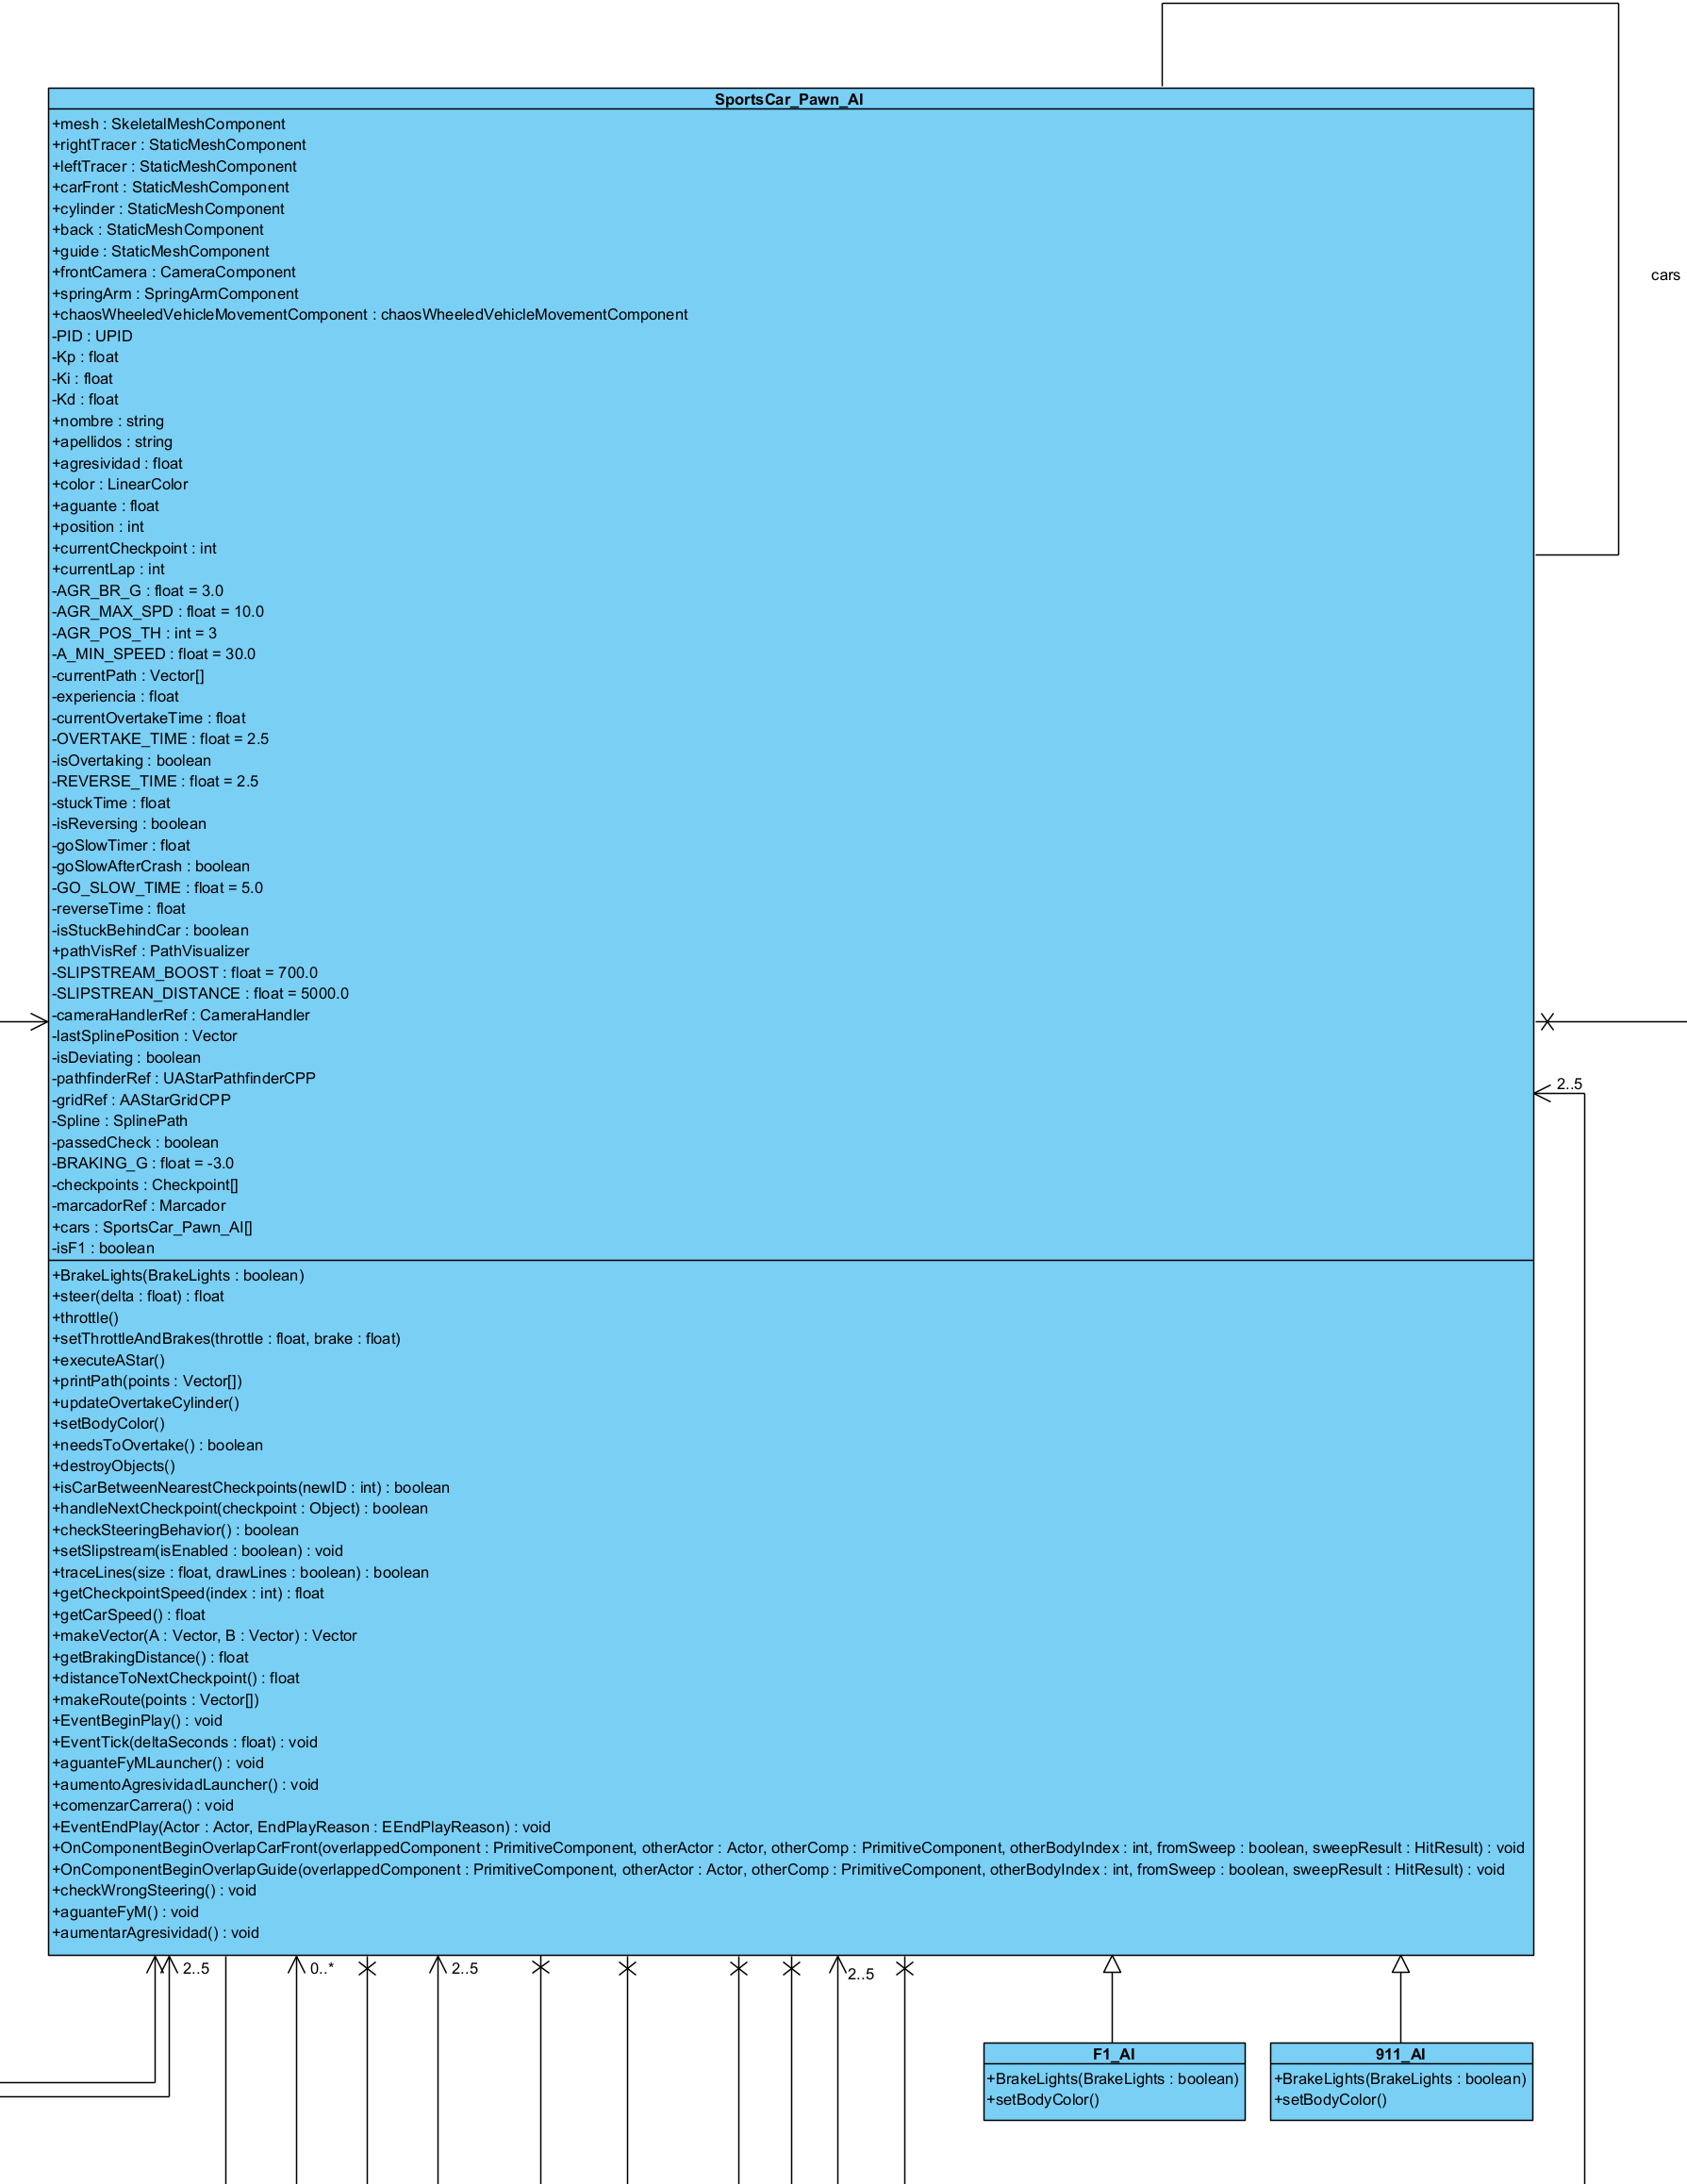
\includegraphics[width=\textwidth]{imagenes/classDiagram1.png}
    \caption{Primera sección del diagrama de clases.}
\end{figure}

\begin{figure}[H]
    \centering
    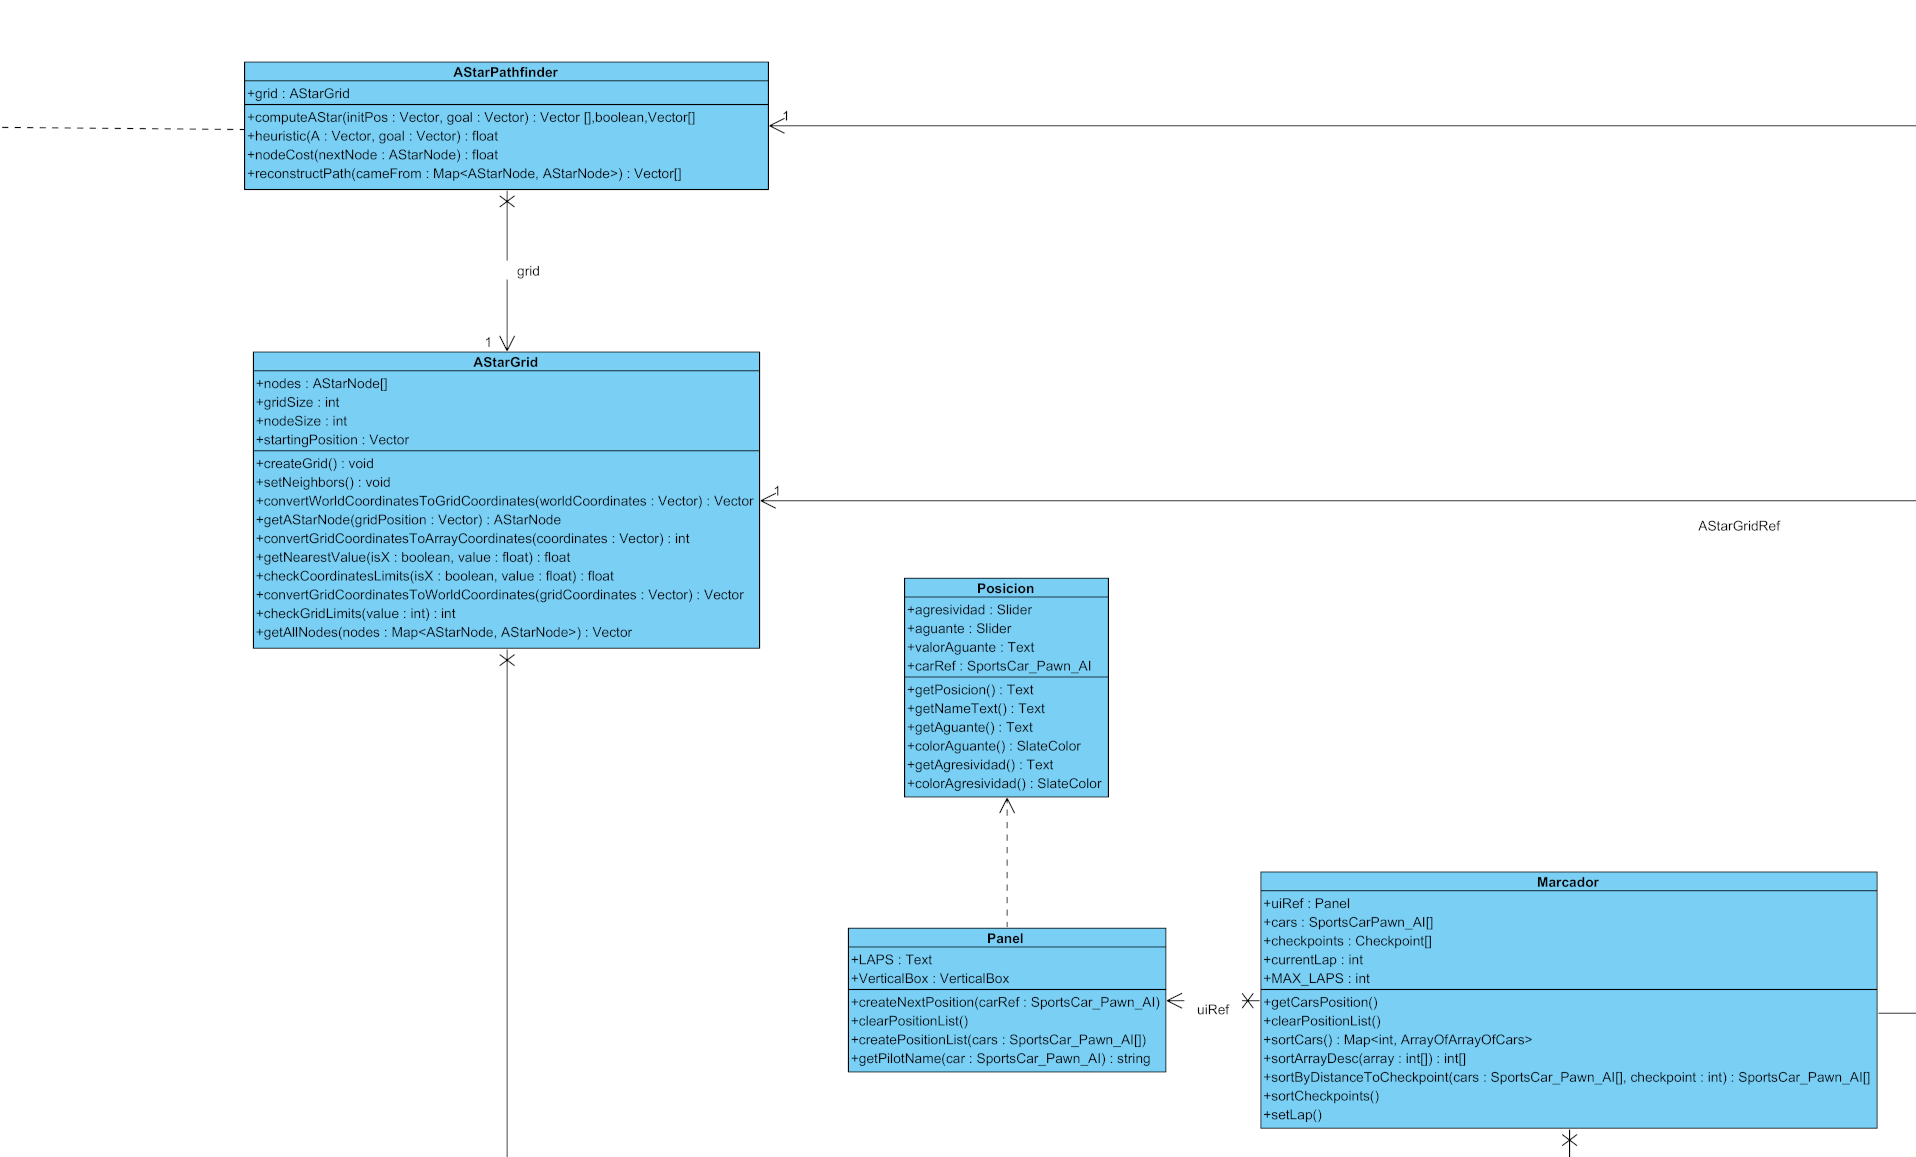
\includegraphics[width=\textwidth]{imagenes/classDiagram2.png}
    \caption{Segunda sección del diagrama de clases.}
\end{figure}

\begin{figure}[H]
    \centering
    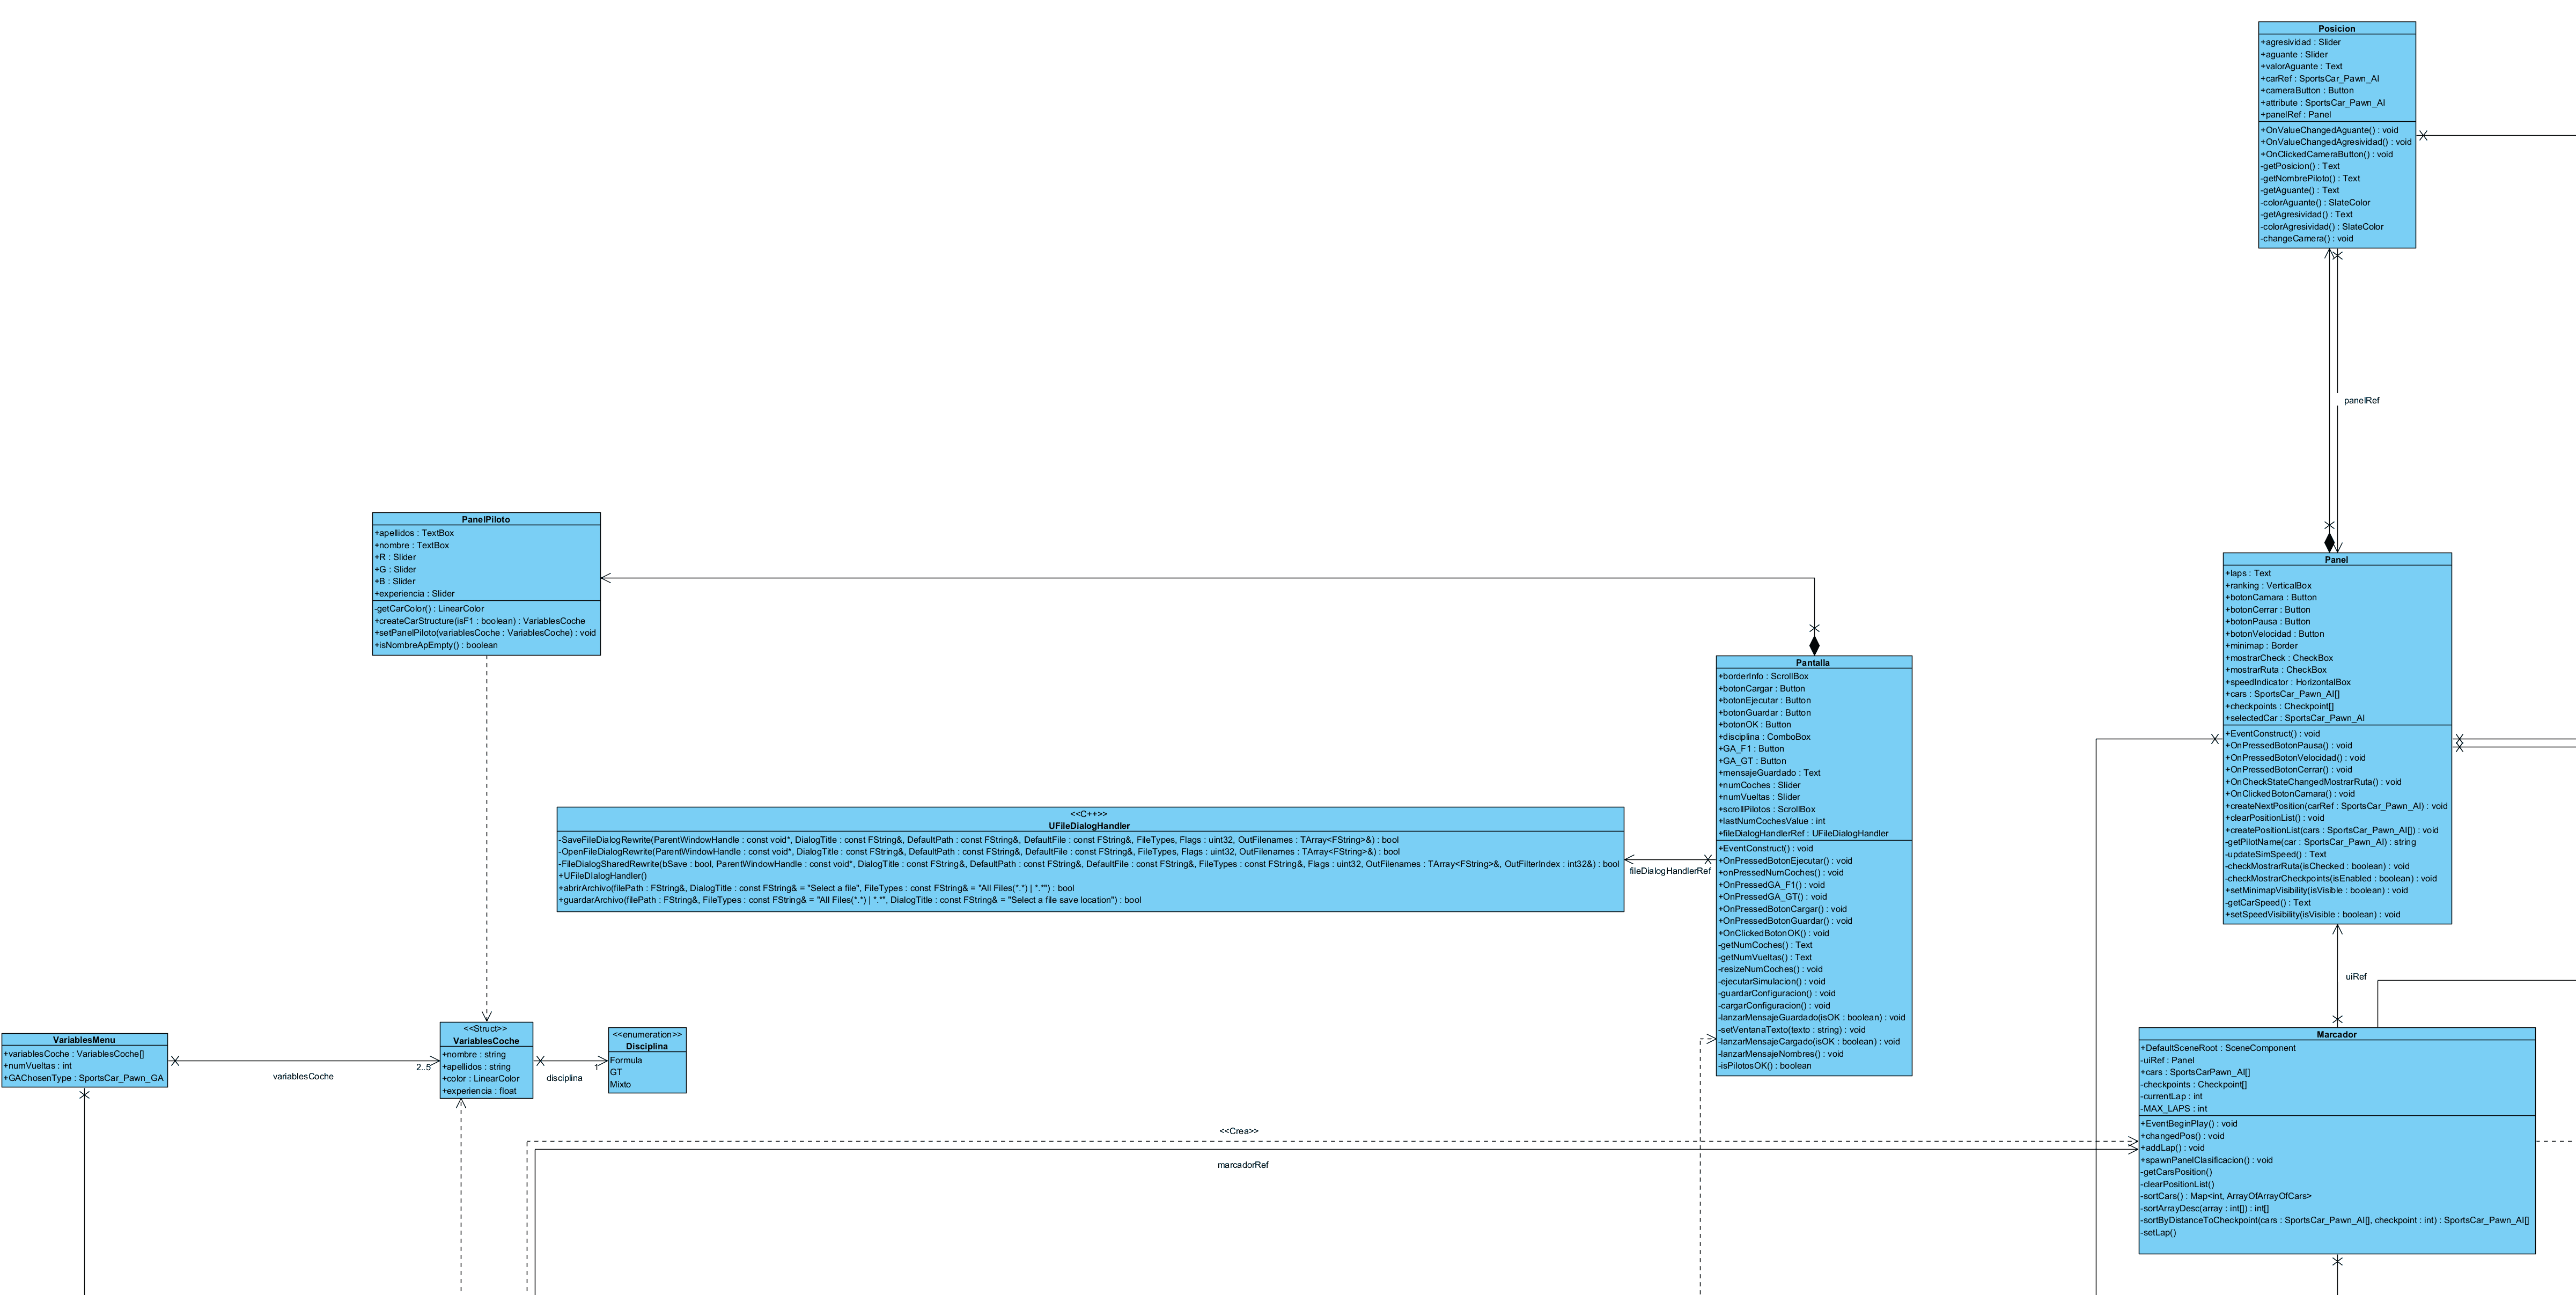
\includegraphics[width=\textwidth]{imagenes/classDiagram3.png}
    \caption{Tercera sección del diagrama de clases.}
\end{figure}

\begin{figure}[H]
    \centering
    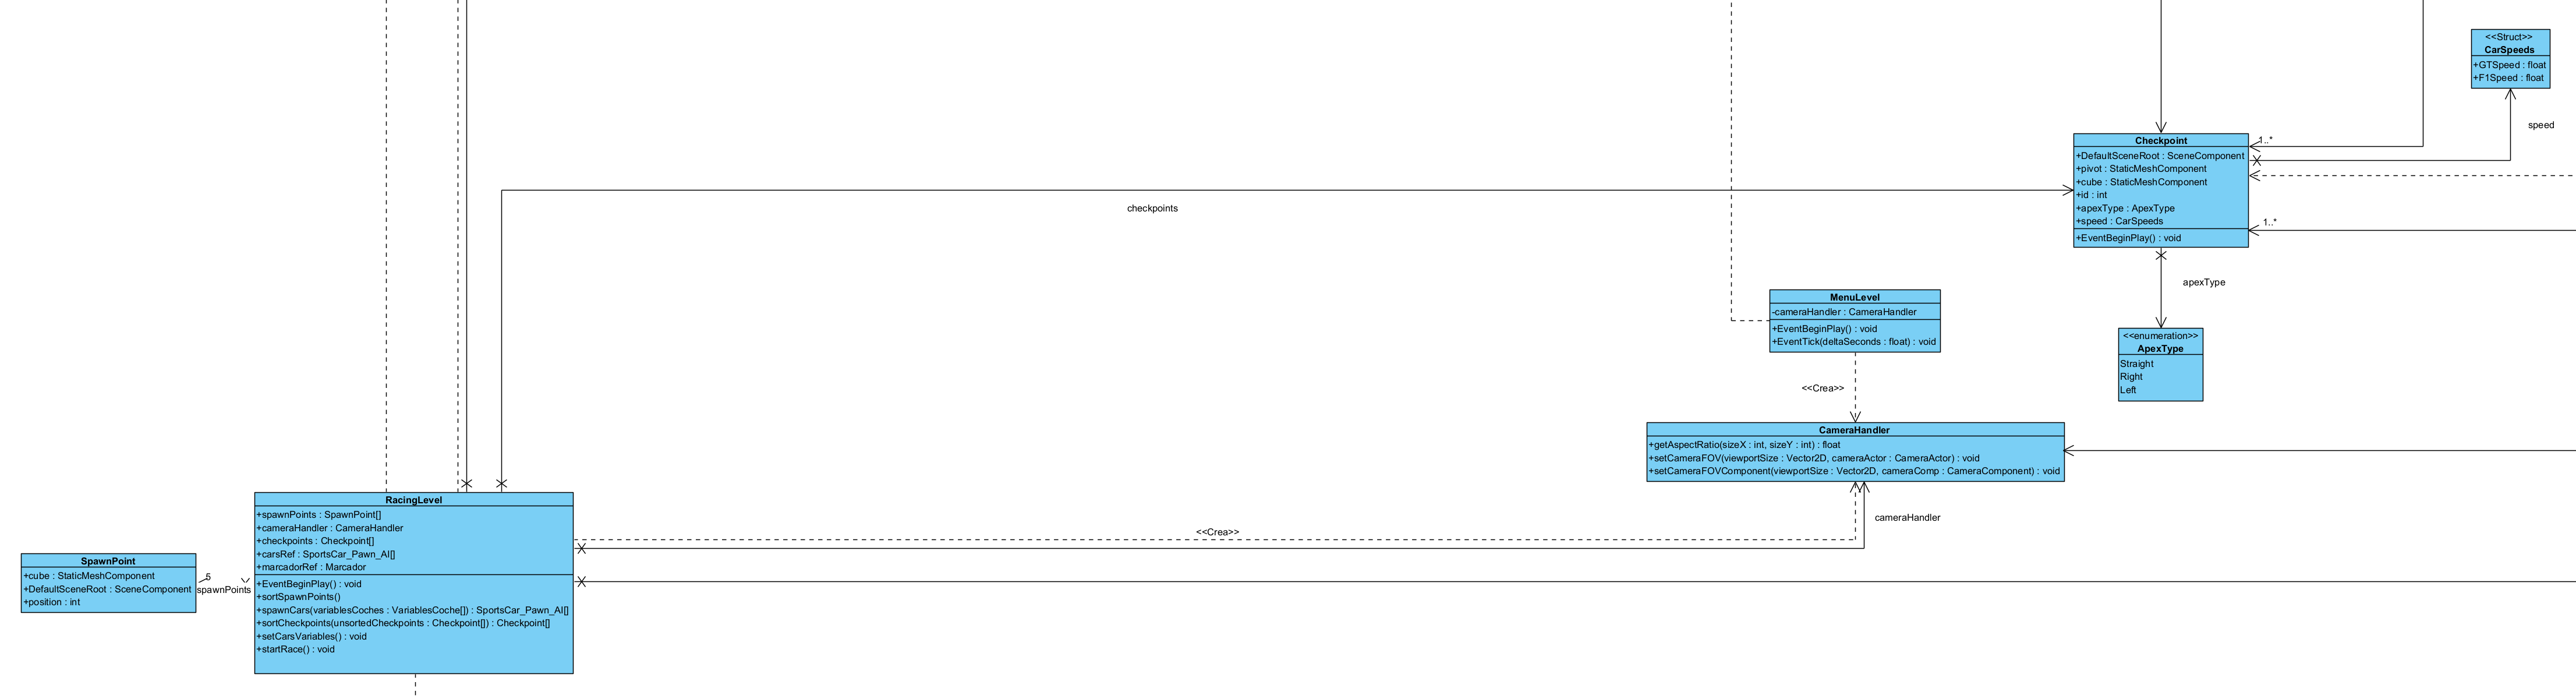
\includegraphics[width=\textwidth]{imagenes/classDiagram4.png}
    \caption{Cuarta sección del diagrama de clases.}
\end{figure}

\section{Diseño de la Interfaz de Usuario}

La interfaz de usuario del configurador de la simulación (el prototipo se puede ver en la figura \ref{fig:protoconfig}) está dividida en dos secciones principales: a la izquierda se encuentra la sección para el número de vehículos y de pilotos, la disciplina y las opciones de importación y exportación de la configuración. A la derecha está la segunda sección, compuesta por las características de cada piloto y el botón para comenzar la simulación.

\begin{figure}[H]
    \centering
    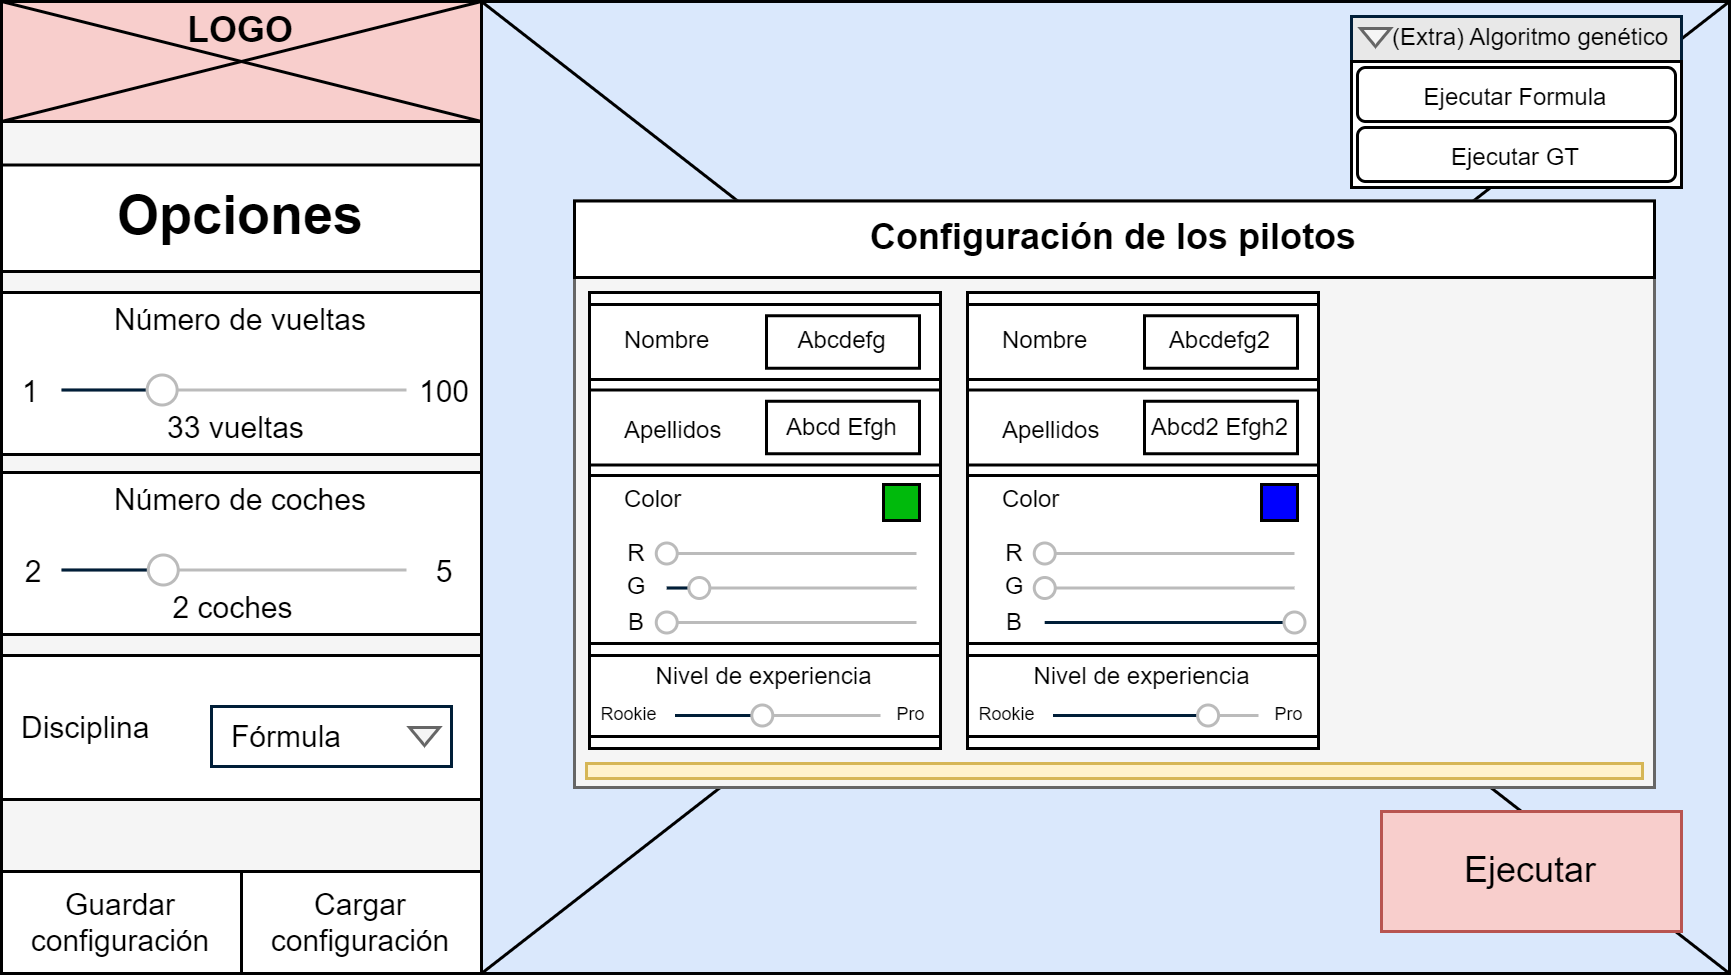
\includegraphics[width=0.7\textwidth]{imagenes/pag1.png}
    \caption{Interfaz del configurador antes de la carrera.}
\end{figure}

Durante la carrera, se mostrará un listado de posiciones de los pilotos y un contador de vueltas (prototipo en la figura \ref{fig:protoranking}) en la parte izquierda de la pantalla. Este listado permitirá visualizar y modificar el estado de cada piloto en tiempo real. La disposición de los elementos será similar a la de disciplinas como la Fórmula 1, donde el ranking de pilotos y el contador de vueltas aparecen a la izquierda, y en cada celda de posición aparecen las tres primeras letras del apellido. En este proyecto, he decidido añadir también la primera letra del nombre, en caso de que haya varios pilotos con el mismo apellido.


\begin{figure}[H]
    \centering
    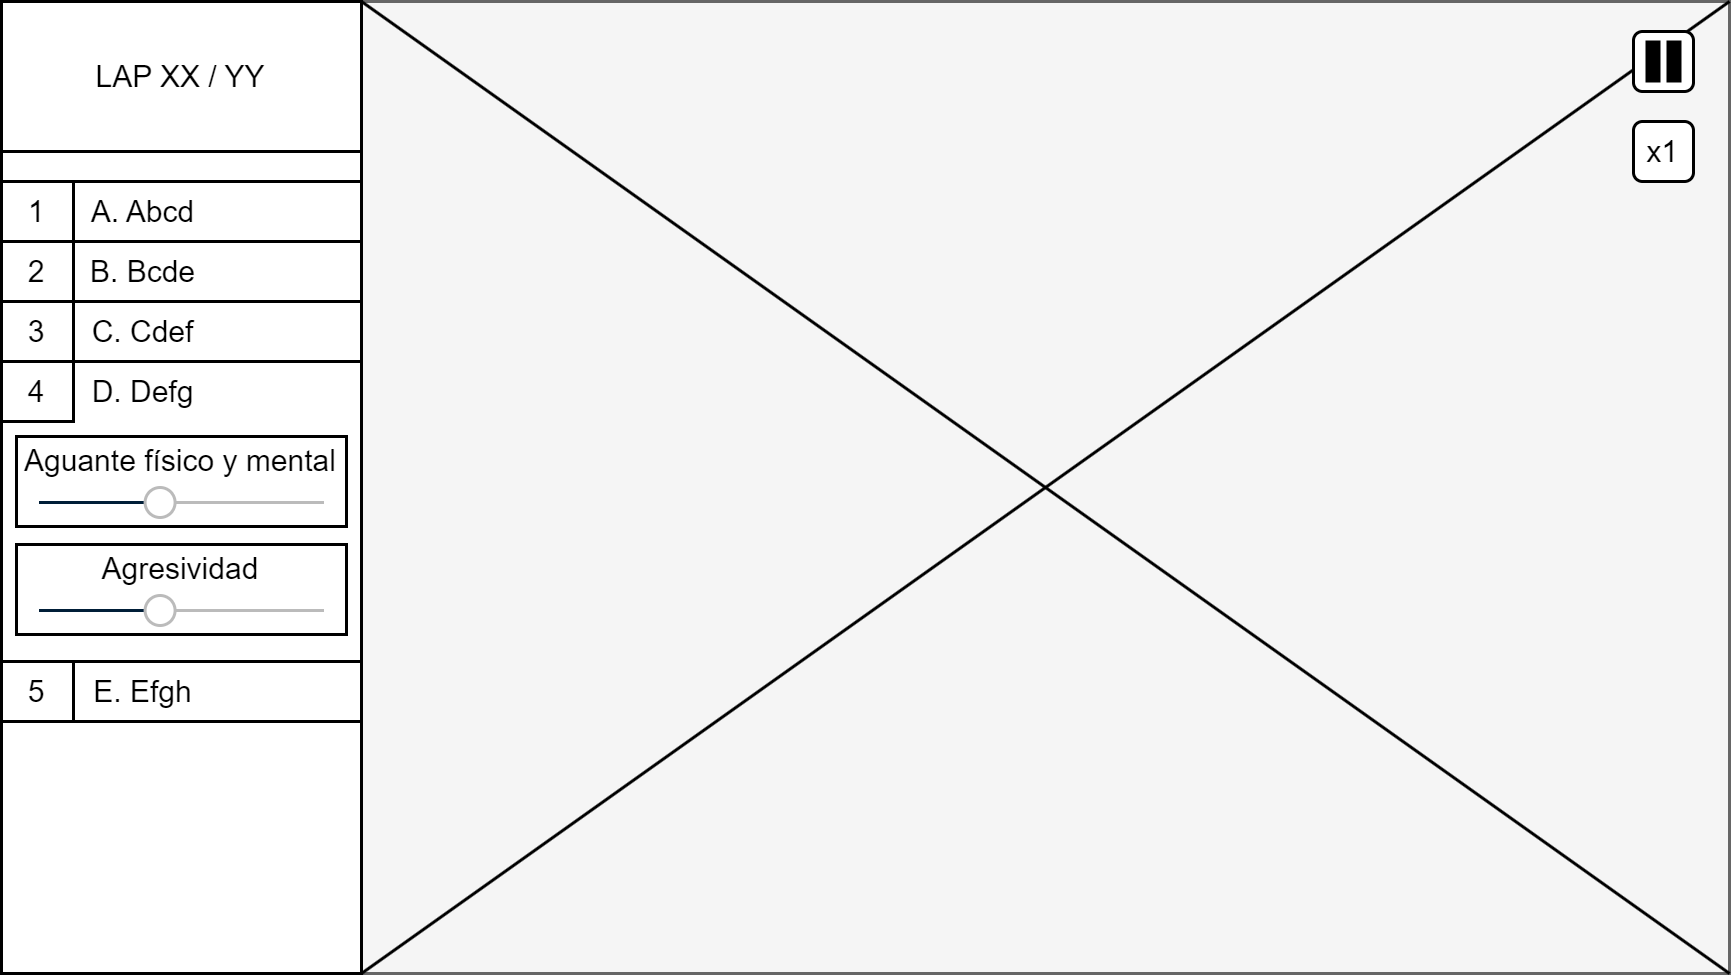
\includegraphics[width=0.7\textwidth]{imagenes/pag2.png}
    \caption{Interfaz de las opciones durante la carrera.}
\end{figure}

\section{Diagrama de navegación}

La navegación por la interfaz de usuario en la aplicación es relativamente sencilla, al estar formada por dos pantallas: el configurador de simulación y la carrera en curso.

\bigskip

El diagrama de navegación de la aplicación se encuentra a continuación:

% foto del diagrama de navegacion
\begin{figure}[H]
    \centering
    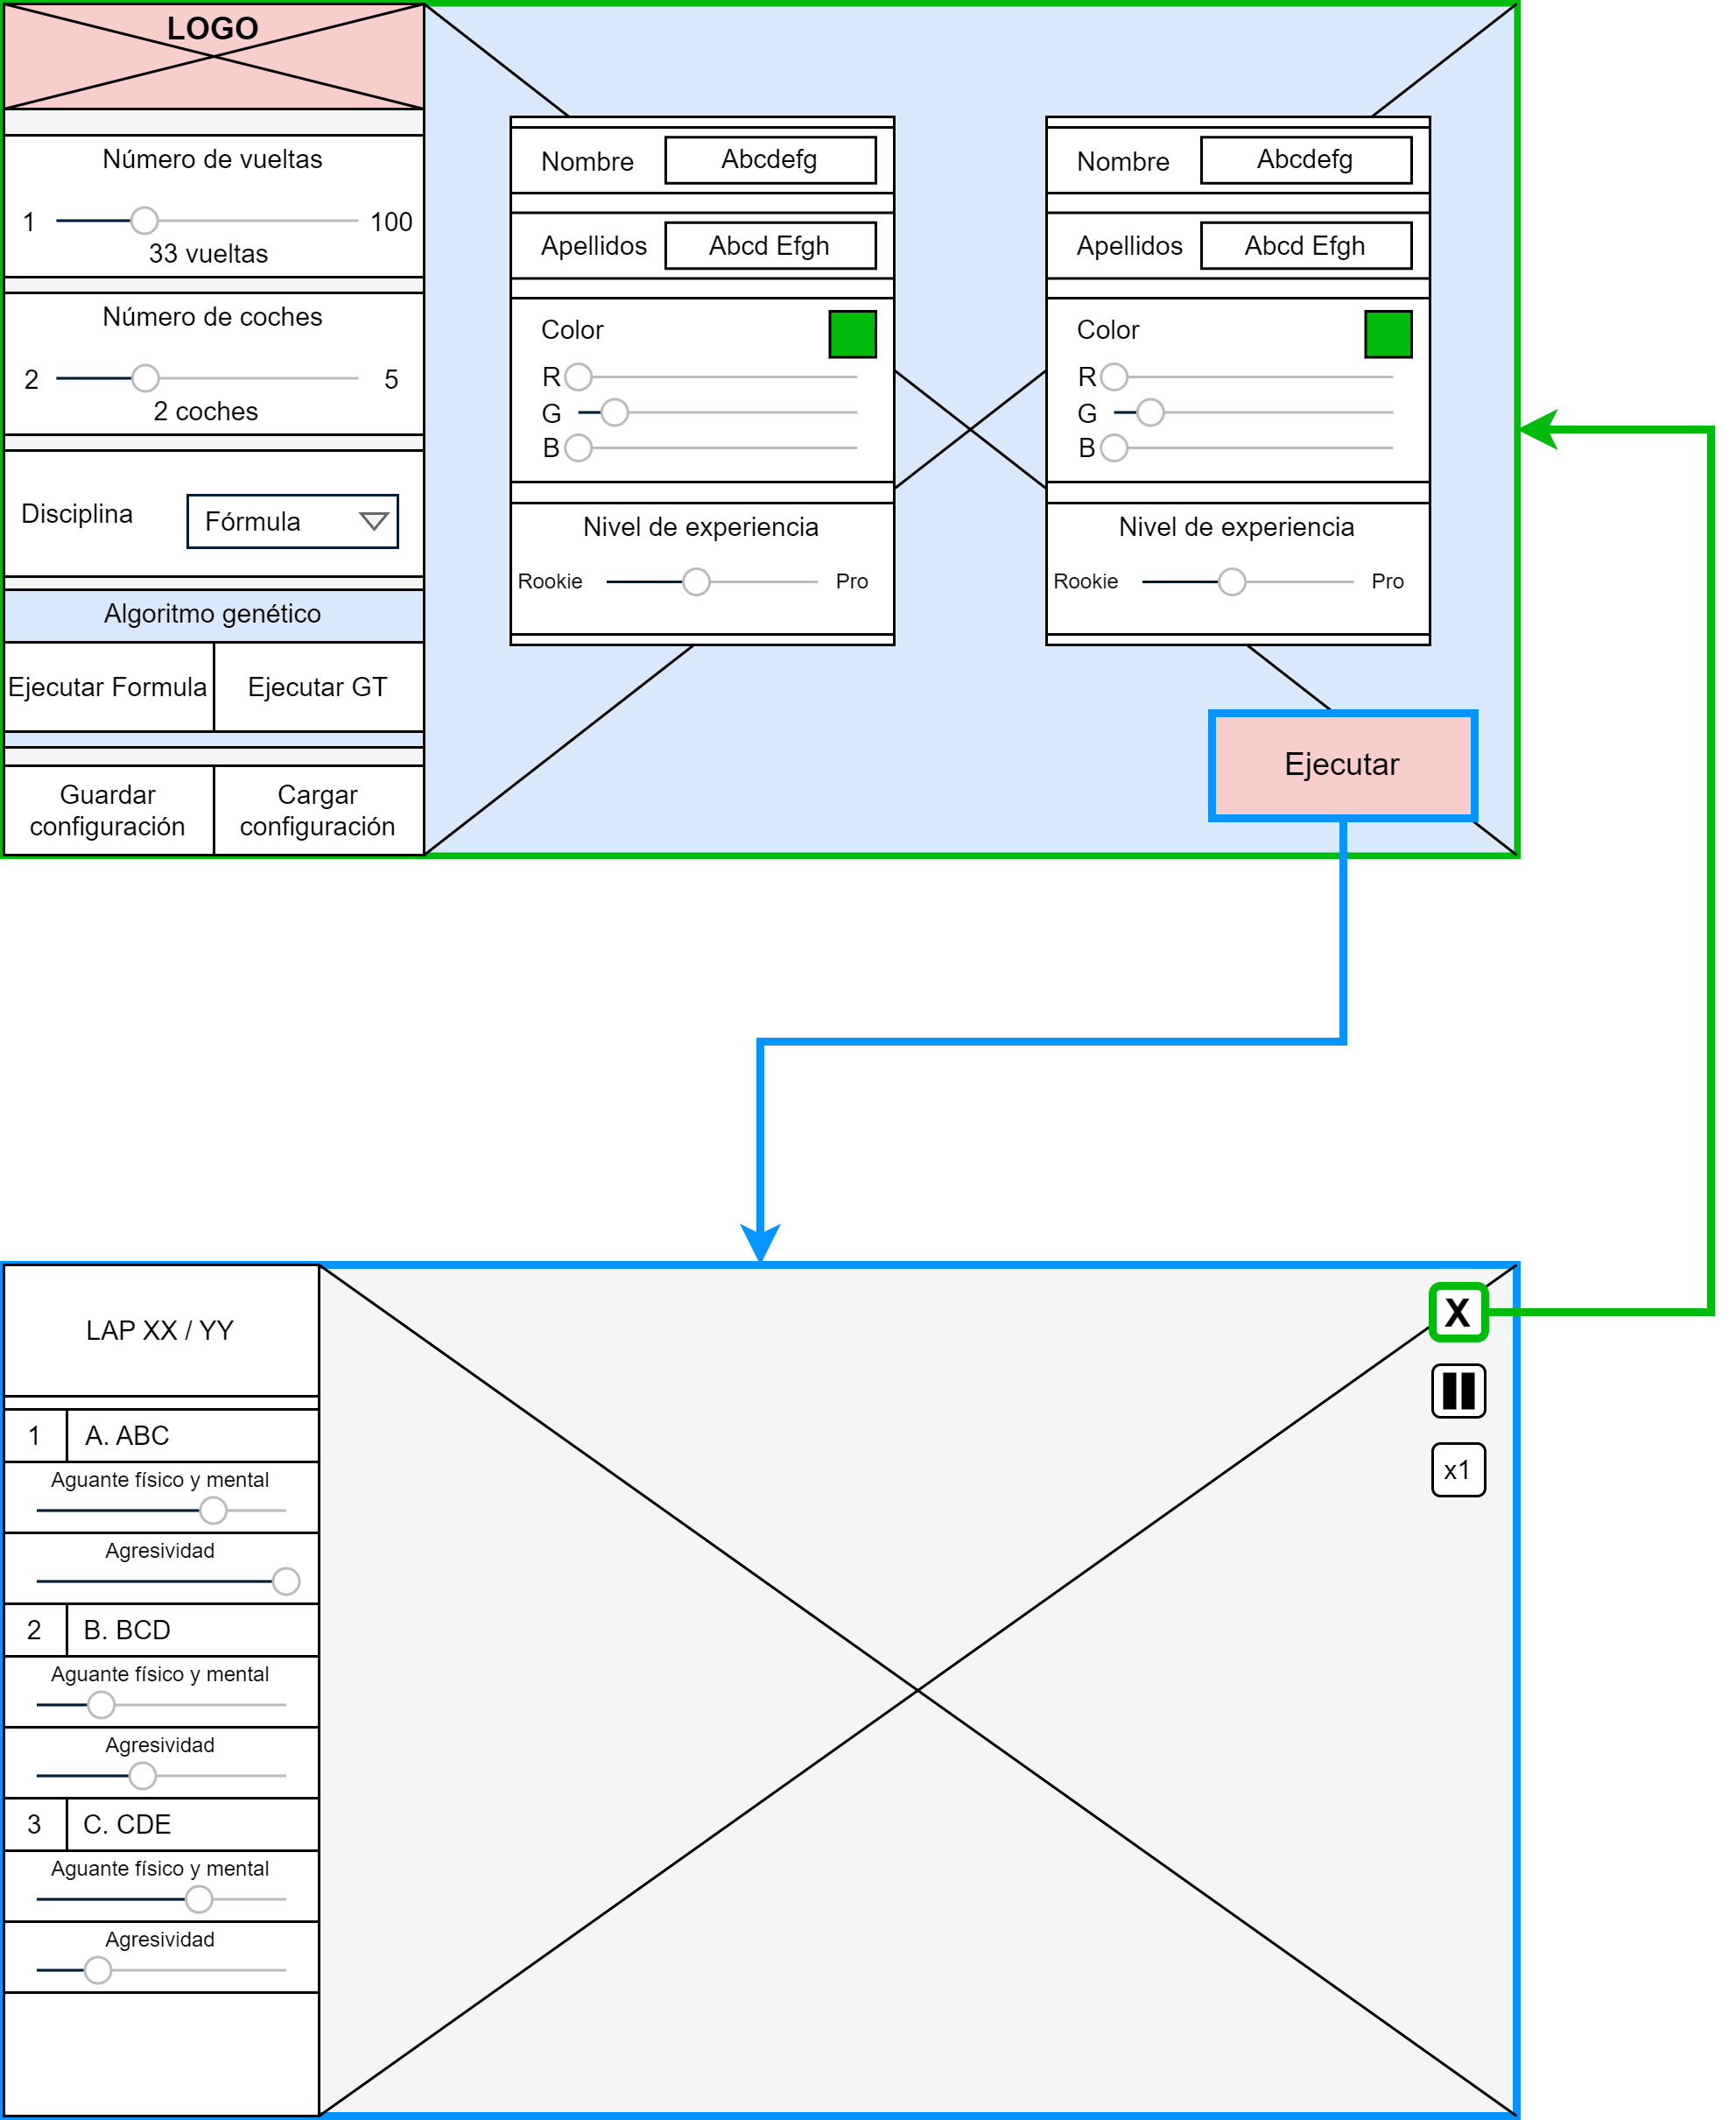
\includegraphics[width=0.9\textwidth]{imagenes/nav.png}
    \caption{Diagrama de navegación de la interfaz de usuario de la aplicación.}
\end{figure}

Como se puede observar en el diagrama de navegación, al pulsar el botón de ejecutar aparecerá la nueva pantalla para ejecutar la simulación y dar comienzo a la carrera. Asimismo, si se pulsa el botón con el símbolo ``X'', se cerrará la simulación en curso y aparecerá de nuevo el configurador.
